\documentclass[Main]{subfiles}
\begin{document}

\subsection{SekvensDiagrammer}

\subsubsection{Use Case 1 -- System initialisering}

\begin{figure}[H]
\centering
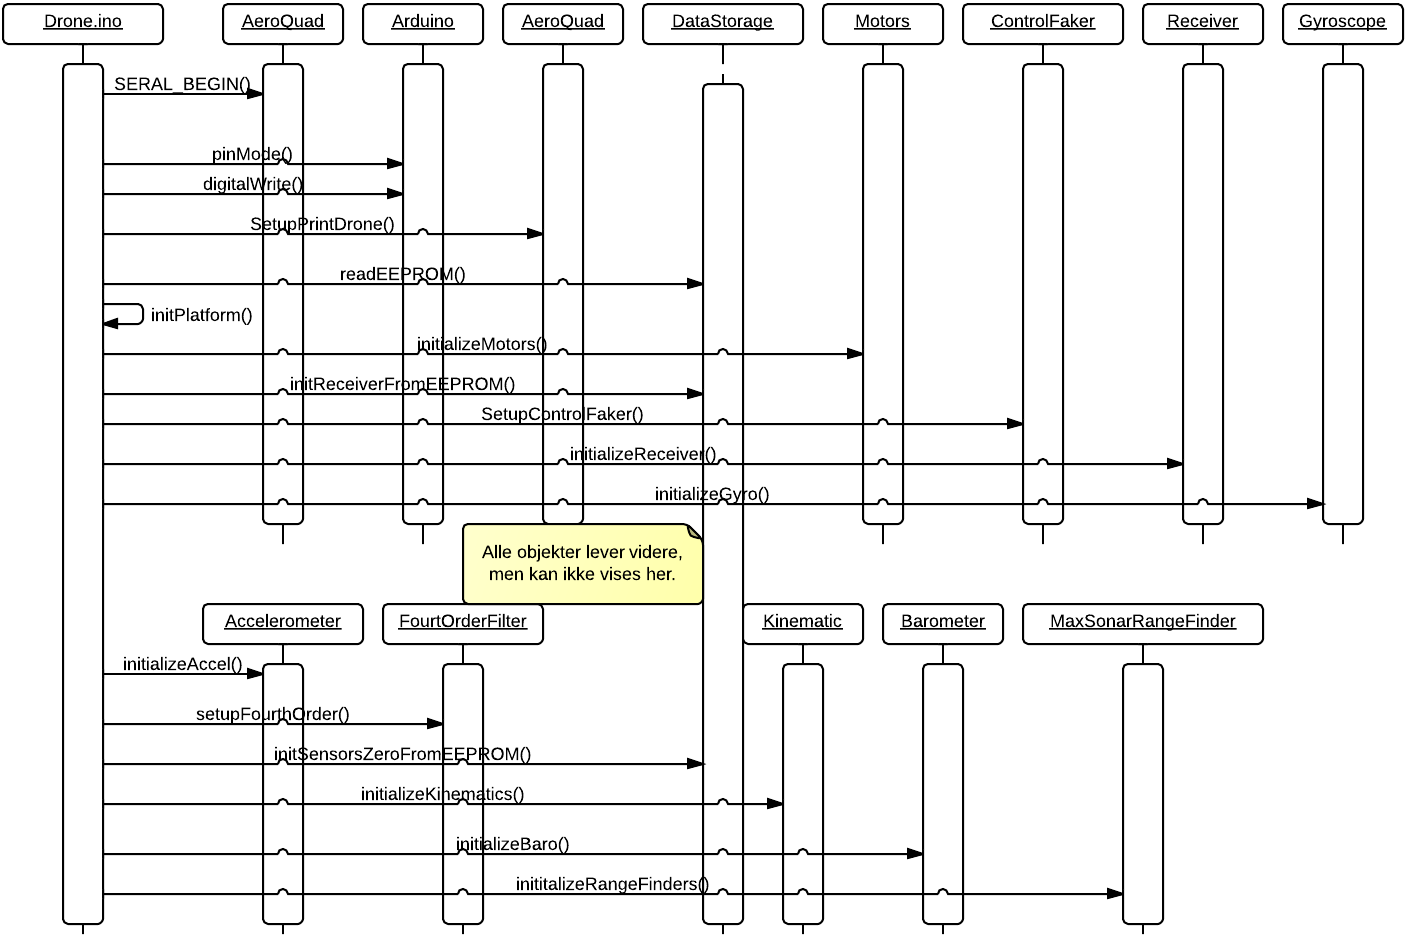
\includegraphics[angle=90, scale = 0.55]{SekvensInit}
\caption{Init af drone}
\label{Fig:SekvInit}
\end{figure}

På Figur \ref{Fig:SekvInit} ses de kald der foretages, når dronen starter op første gang den får strøm.
Efter initieringen startes Arduino's \code{loop()}-funktion, der kører i ring til strømmen afbrydes, som vist på Figur \ref{Fig:SekvDroneHz}.


\begin{figure}[H]
\centering
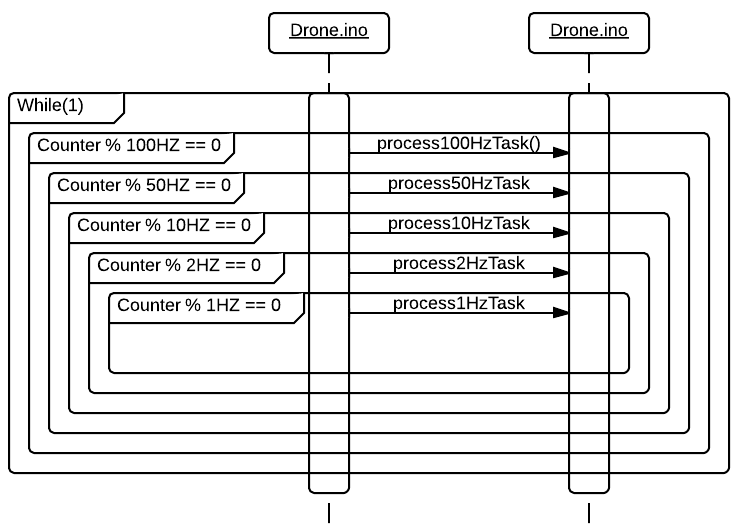
\includegraphics[scale=0.55]{DroneLoop}
\caption{Schedulering i \code{loop()}-funktionen}
\label{Fig:SekvDroneHz}
\end{figure}

Input til, hvordan dronen skal flyve, bliver registreret i \code{50HzTask()} og er illustreret på Figur \ref{Fig:50Hz}.

\begin{figure}[H]
\centering
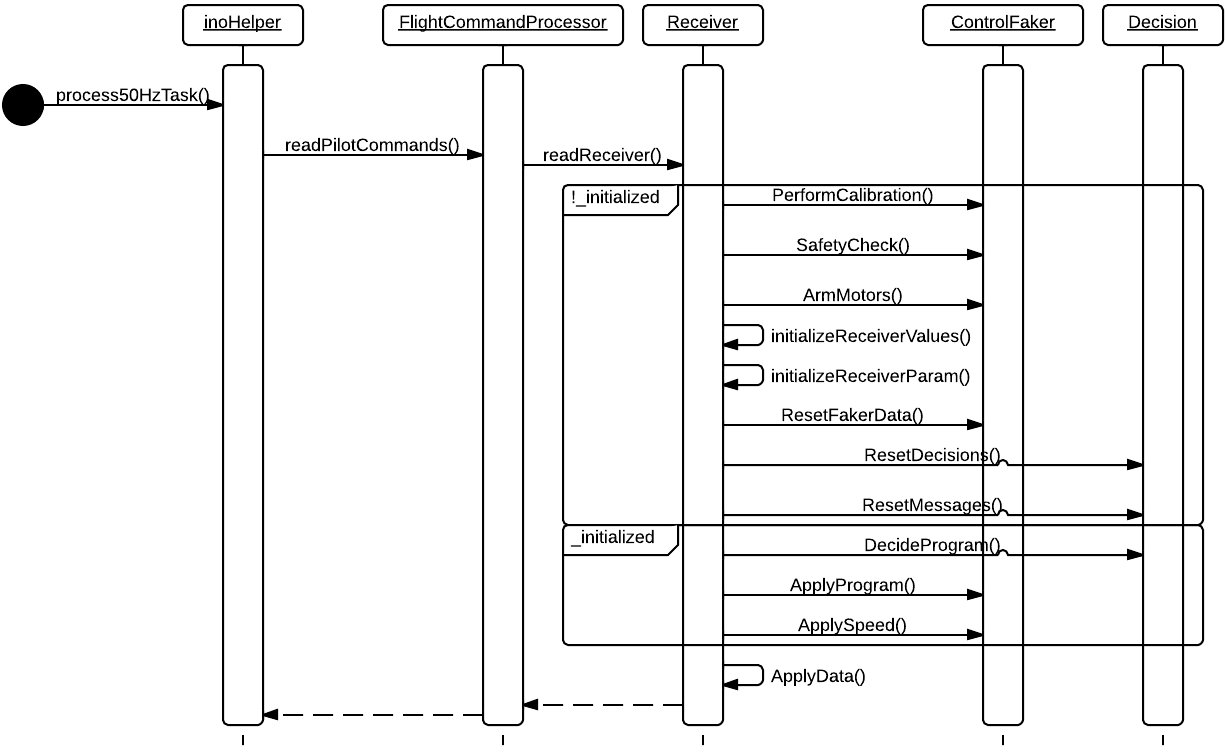
\includegraphics[width = \textwidth]{50HzProcess}
\caption{50 Hz processen. \textbf{Skal der være nummer på hver funktion?}}
\label{Fig:50Hz}
\end{figure}

Når kalibreringen og sikkerhedstjekket er kørt igennem, nulstilles \code{Receiver}'ens lokale værdier, samt \code{ControlFaker}'ens og \code{Decision}'s lokale værdier.
Nu er dronen klar til at flyve.

Herefter vælges hvilket program der skal køres, der pga. nulstillingen er default-programmet, vil få dronen til at spinne med minimal hastighed, hvilket først læser det aktuelle programs data, sætter hastighed og derefter eksekverer dataene.


\newpage
\subsubsection{Use Case 2 -- Programvalg}
Når brugeren af systemet vælger et program, sendes signalet fra fjernbetjeningen til dronens radiomodtager, der læses af \code{DecideProgram()} (fra Figur \ref{Fig:50Hz}) og er illustreret på Figur \ref{Fig:SendProgram} og Figur \ref{Fig:DecideProgram}.

\begin{figure}[H]
\centering
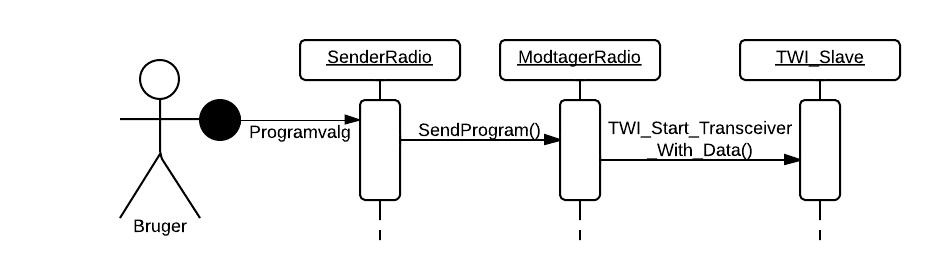
\includegraphics[width = \textwidth]{SendProgram}
\caption{Skriv til radio.}
\label{Fig:SendProgram}
\end{figure}


\begin{figure}[H]
\centering
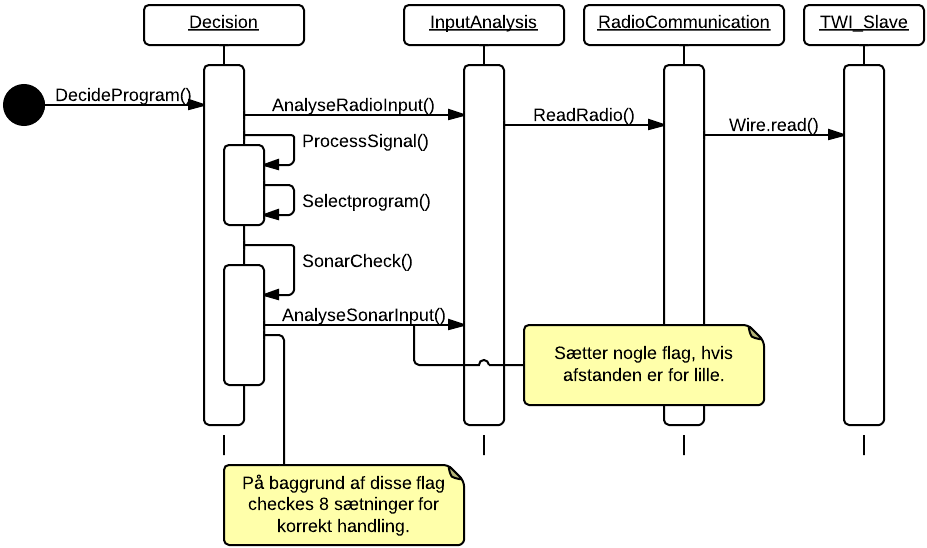
\includegraphics[width = \textwidth]{DecideProgram}
\caption{Læs radio.}
\label{Fig:DecideProgram}
\end{figure}


\newpage
\subsubsection{Use Case 3 -- Sonaradvarsel.}
Når dronen flyver kan de 3 sonarsensorer, der sidder foran den, registrere hvor langt der er til nærmeste objekt i en kegle 67$^{\circ}$.\fxnote{Reference til hardware afsnit samt beregninger}
Såfremt de registrerer noget (på et gennemsnit af de seneste to målinger), vil et flag blive sat, hvilket checkes for i \code{DecideProgram()} (fra Figur \ref{Fig:50Hz})

















\end{document}